\documentclass[a4paper,11pt]{article}

\usepackage[T1]{fontenc} \usepackage{lmodern} \usepackage[utf8]{inputenc}
\usepackage[english]{babel} \usepackage{csquotes}
\usepackage{float} \usepackage{graphicx,subfigure}
\usepackage{amssymb,amsmath,epstopdf} %\usepackage{siunitx}
\usepackage[nodayofweek]{datetime}
\usepackage[top=3.0cm,bottom=2.0cm,left=2.5cm,right=2.5cm,headheight=30pt]{geometry}
\usepackage{natbib} 
\usepackage{fancyhdr} \pagestyle{fancy} \usepackage{lastpage}
\usepackage{parskip} \setlength{\parskip}{.5em} \setlength{\parindent}{1em}
\usepackage[colorlinks=true,allcolors=blue]{hyperref} \hypersetup{
	pdfauthor={Michaël Defferrard, Soroosh Shafiee},
	pdftitle={Incremental Gradient Methods},
	pdfsubject={Project proposal}
}
\lhead{Advanced Topics in Data Sciences\\ Project report}
\chead{\hspace{2cm}EPFL\\ \hspace{2cm}\shortdate\today}
\rhead{Michaël \textsc{Defferrard}\\ Soroosh \textsc{Shafiee}}
\cfoot{}

\newcommand{\R}{\mathbb{R}}
\newcommand{\B}{\mathcal{B}}
\newcommand{\eqnref}[1]{(\ref{eqn:#1})}
\newcommand{\figref}[1]{Figure~\ref{fig:#1}}
\newcommand{\prox}{\textrm{prox}}
%\DeclareMathOperator*{\prox}{prox}

\begin{document}

\begin{center}
	\Large{\textbf{\textsc{Incremental Gradient Methods}}}
\end{center}

This project is aimed to be a way for us to better understand and thinker with
the recent advances in Stochastic Gradient Descent algorithms, specifically
the recent SAGA \cite{defazio_saga_2014}. This method is similar in spirit to
the previously developed SAG, SDCA, MISO and SVRG. This class of algorithms have
been developed to solve problems of the form
\begin{equation} \label{eqn:problem}
	\min_{x \in \R^d} \frac{1}{n} \sum_{i=1}^n f_i(x) + h(x),
\end{equation}
where each $f_i$ is convex and has Libschitz continuous derivatives with
constant $L$ or is strongly convex with constant $\mu$; and $h$ is a convex but
potentially non-differentiable function (his proximal operator is however easy
to compute). While computing the full gradient would be prohibitive due to large
$d$ and $n$, these iterative stochastic algorithms reduce the computational cost
of optimization by only computing the gradient of a subset of the functions
$f_i$ at each step.

Many machine learning problems can be cast in \eqnref{problem}, such as
(constrained) Least-Square or Logistic Regressions with $\ell_1$ or $\ell_2$
regularization; where $x$ would represent the model parameters, $f_i$ the data
fidelity term applied to a particular sample $i$, and $h$ a regularization or
indicator function of a convex set.

In this project we explored two approaches to improve SAGA towards two different
goals:
\begin{itemize}
	\item A \textbf{memory-efficient SAGA}, by way of computing and storing
		gradients over mini-batches instead of single samples, as is done for
		the infamous Stochastic Gradient Descent \cite{konevcny2014ms2gd}. It turns out that this
		approach is also faster than the original algorithm as it exploits the
		vectorial capabilities of modern processing units.
	\item A \textbf{time-efficient SAGA}, by way of distributing the gradient
		computation over many CPU cores while fusing the results and updating
		the model parameters on the master. The similar approach is also presented in \cite{lee2015distributed} for SVRG algorithm.
\end{itemize}

\section{SAGA algorithm} \label{sec1}

The algorithm starts with some known initial vector $x^0 \in \R^d$ and known
derivatives $f_i' (\phi_i^0) \in \R^d$ with $\phi_i^0 = x^0$ for each $i$. These
derivatives are stored in a table data-structure of length $n$, or alternatively
a $n \times d$ matrix. It uses a step size of $\gamma$\footnote{The authors
recommend a learning rate of $\gamma=1/(2(\mu n+L))$ in the strongly convex
case, $\gamma=1/(3(\mu n+L))$ if the strong convexity requirement only holds on
average and $\gamma=1/(3L)$ for non-strongly convex problems.} and, given the
value of $x^k$ and of each $f_i' (\phi_i^k)$ at the end of iteration $k$, makes
the following updates for iteration $k+1$:
\begin{enumerate}
\item Pick a $j$ uniformly at random.
\item Take $\phi_j^{k+1} = x^k$, and store $f_j'(\phi_j^{k+1})$ in the table.
	All other entries in the table remain unchanged. The quantity $\phi_j^{k+1}$
	is not explicitly stored.
\item Update $x$ using $f_j'(\phi_j^{k+1})$, $f_j'(\phi_j^k)$ and the table
	average:
	\begin{equation} \label{eqn:saga}
	w^{k+1} = x^k - \gamma \left[ f_j'(\phi_j^{k+1}) - f_j'(\phi_j^k)
	+ \frac1n \sum_{i=1}^n f_i'(\phi_i^k) \right] ,
	\end{equation}
	$$x^{k+1} = \prox_\gamma^h (w^{k+1}).$$
\end{enumerate}

As the authors of \cite{defazio_saga_2014}, we tested our algorithms by training
a linear regression model (with $\ell_1$ or $\ell_2$ regularization) on the
Million Song dataset\footnote{
\url{http://labrosa.ee.columbia.edu/millionsong}}. The problem, as stated on the
UCI repository\footnote{
\url{http://archive.ics.uci.edu/ml/datasets/YearPredictionMSD}} where the data
was downloaded from, is to predict the release year of a song from audio
features.

\section{Mini-batch SAGA}

We first form $\frac{n}m$ mini-batches $\{\B_i\}_{i=1}^{\frac{n}m}$ of size
$|\B_i| = m$ and take gradients w.r.t. them, such that the gradient matrix is of
size $\frac{n}m \times d$ instead of $n \times d$. The updates for iteration
$k+1$ then becomes:
\begin{enumerate}
\item Pick a $i$ uniformly at random in $[1, \frac{n}m]$.
\item Take $\phi_j^{k+1} = x^k \ \forall \ j \in \B_i$, and store $\frac1m
	\sum_{j\in\B_i} f_j'(\phi_j^{k+1})$ in the table.
\item Update $x^{k+1} = \prox_\gamma^h \left\{
	x^k - \gamma \left[ \frac1m \sum_{j\in\B_i} f_j'(\phi_j^{k+1})
	- \frac1m \sum_{j\in\B_i} f_j'(\phi_j^k)
	+ \frac1n \sum_{i=1}^m \sum_{j\in\B_i} f_j'(\phi_j^k) \right] \right\}.$
\end{enumerate}

Note that one can usually vectorize the computation of $\sum_{j\in\B_i}
f_j'(\phi_j^k)$. E.g. for a least-square problem $\min_x \frac12 \|Ax -
y\|_2^2$, the gradient is given by $A_{\B_i}^T A_{\B_i} x$, where $A_{\B_i}$
represents the $m$ columns of $A$ selected by the mini-batch $\B_i$. That is
where the computational advantage of the mini-batch approach comes from.

Note that mini-batches can be formed during initialization and kept intact for
the whole training. They can alternatively be reformed at the beginning of each
training epoch. While this is much more expensive, because the gradient matrix
has to be initialized again, we found no difference in performance.

\subsection{Experiments}

While the convergence rate is the same for all mini-batch sizes given the same
learning rate, larger mini-batches need a smaller learning rate to avoid
divergence.  We therefore ran experiments with various mini-batch sizes $m$;
with an optimized learning rate $\gamma$ for each. \figref{eval_saga_mb} clearly
shows that mini-batch SAGA can outperform regular SAGA in convergence time while
requiring less memory. Other simulation results as well as the problem explanation can be found in Ipython notebook file. This file contains the authors of \cite{defazio_saga_2014} implementation in Cython which is used to assess our implementation.

\begin{figure*}[ht]
	\centering
	\subfigure[Working memory to store gradients.]{
		\label{fig:memory}
		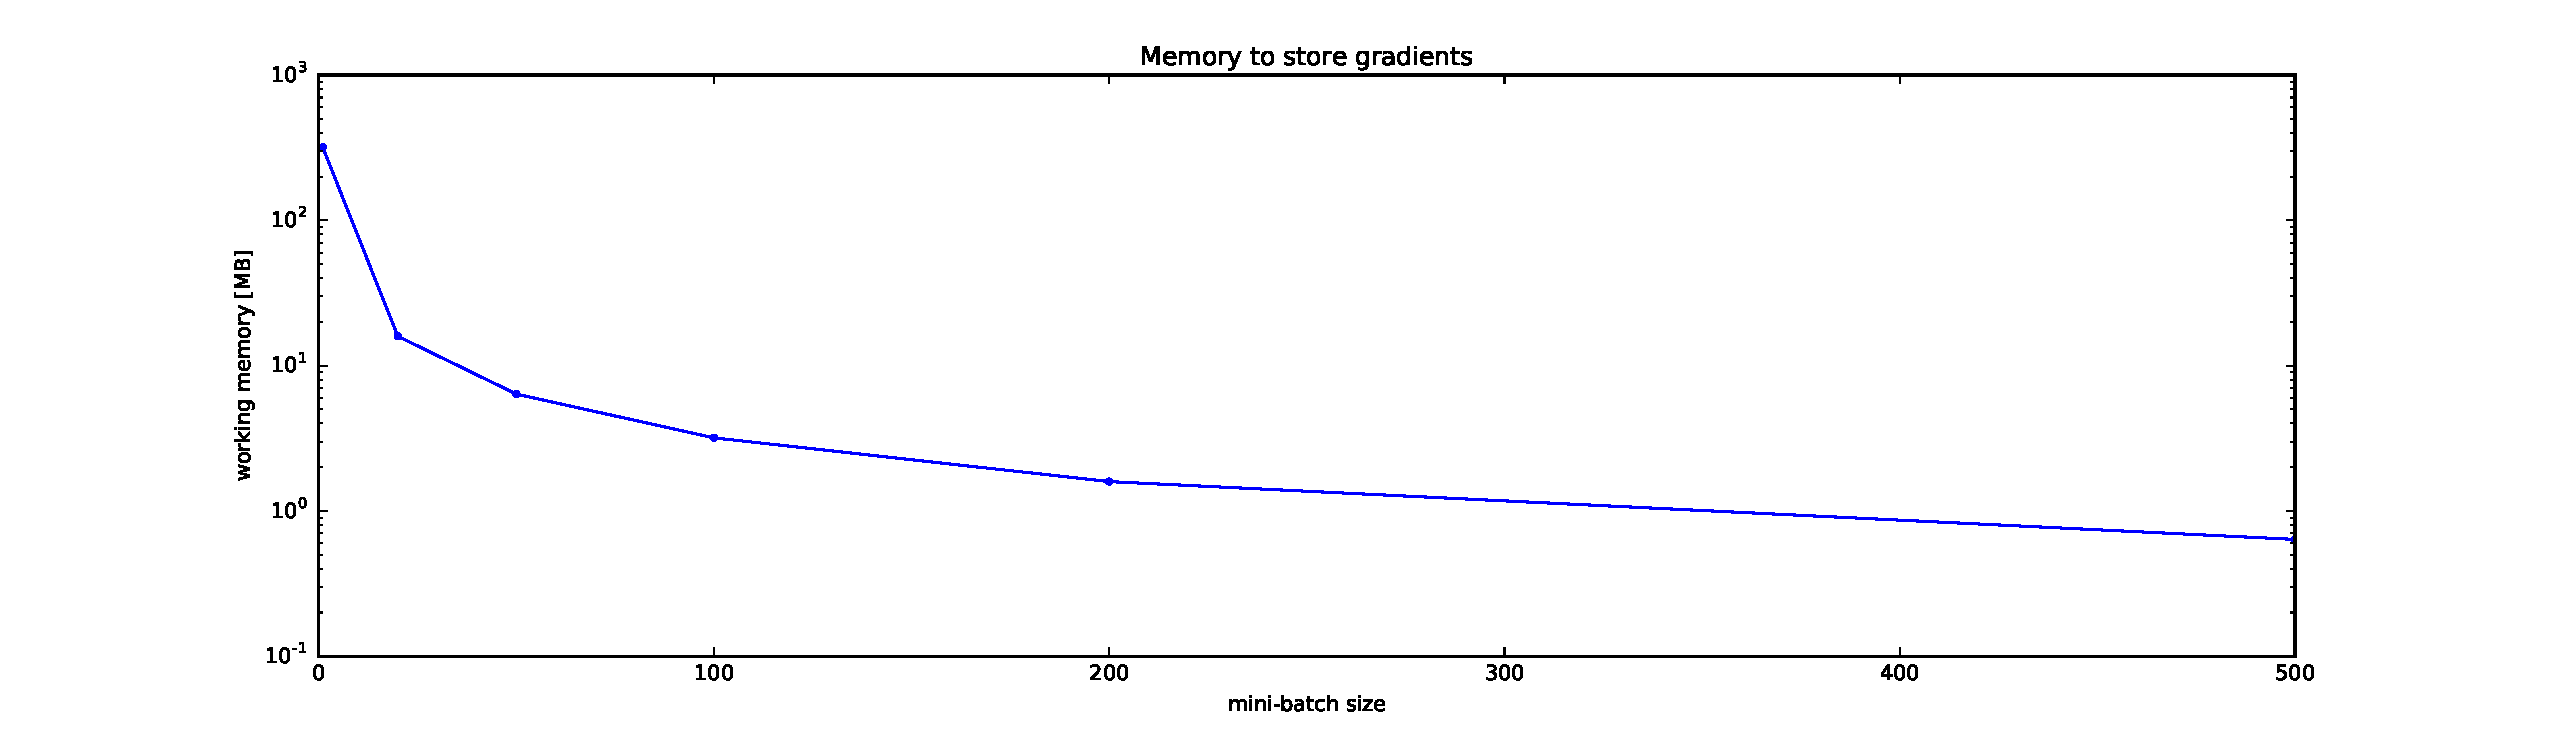
\includegraphics[height=3cm,width=7cm]{figs/memory}}
	\hspace{0pt}
	\subfigure[$R^2$ score on test set after 100s training.]{
		\label{fig:r2_score}
		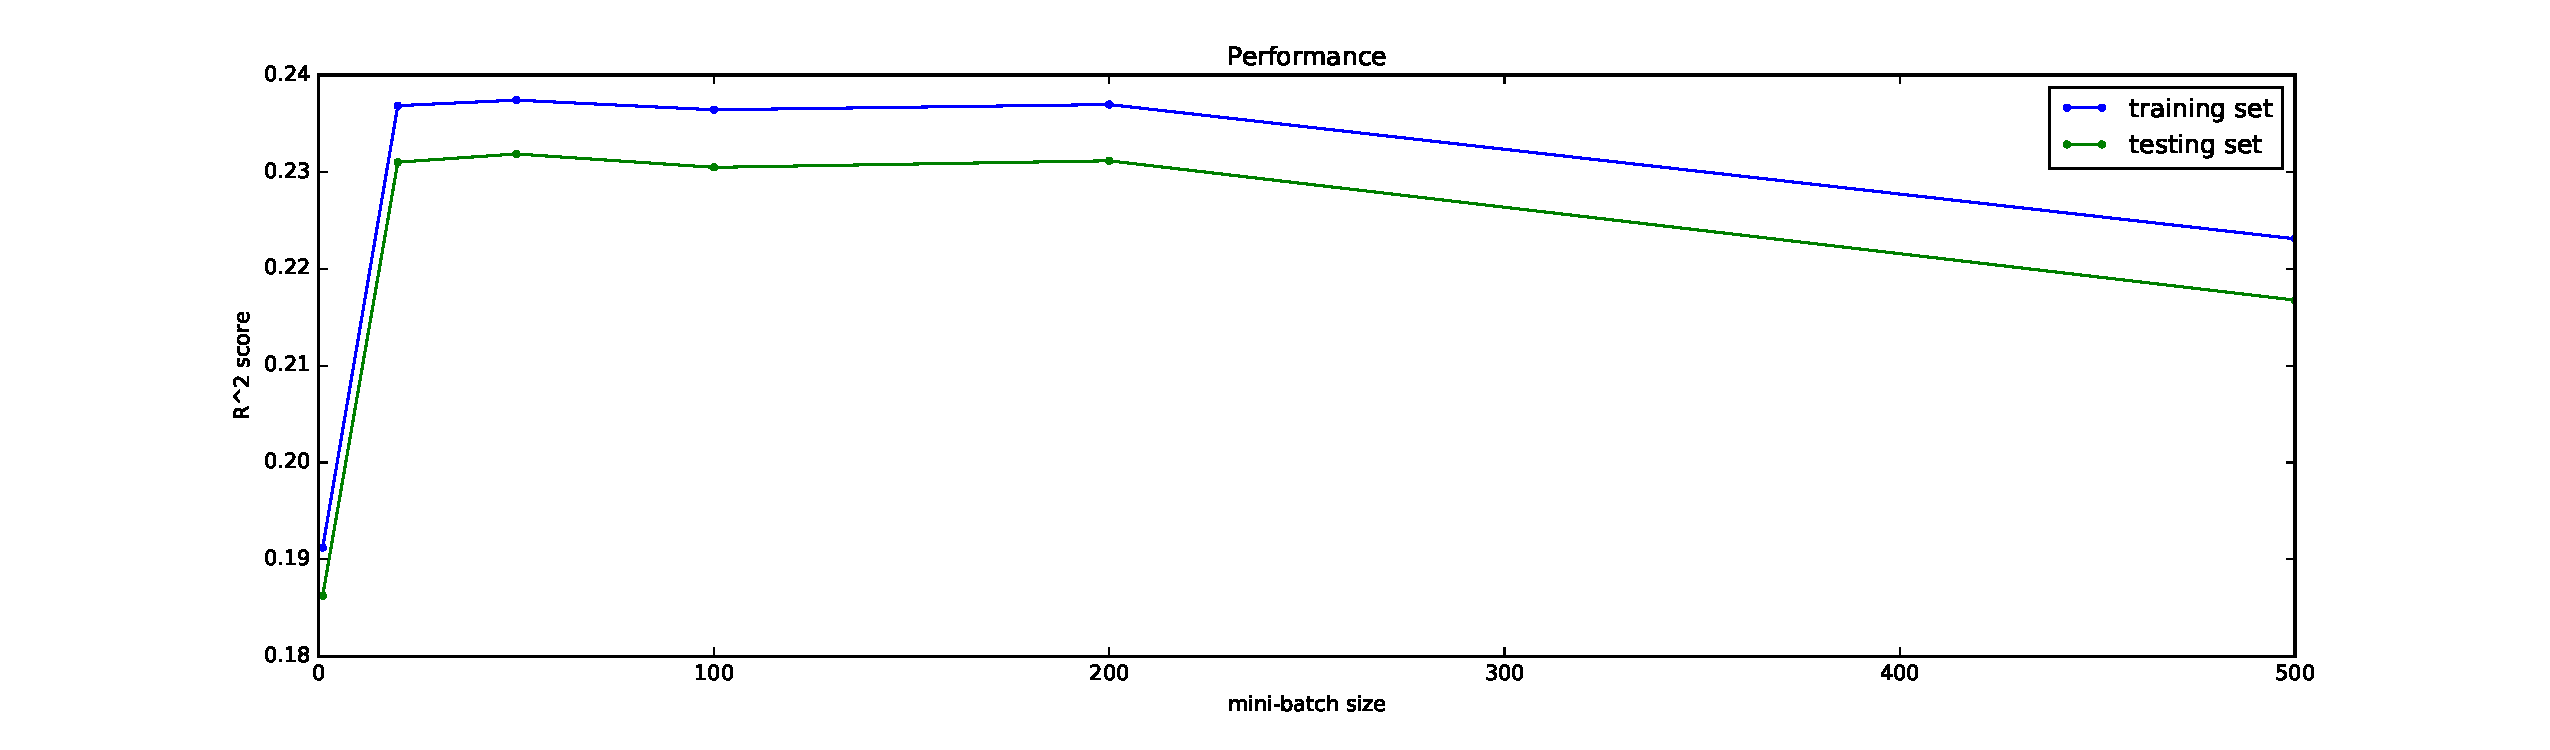
\includegraphics[height=3cm,width=7cm]{figs/r2_score}}
	\\
	\subfigure[Objective w.r.t. running time.]{
		\label{fig:perf}
		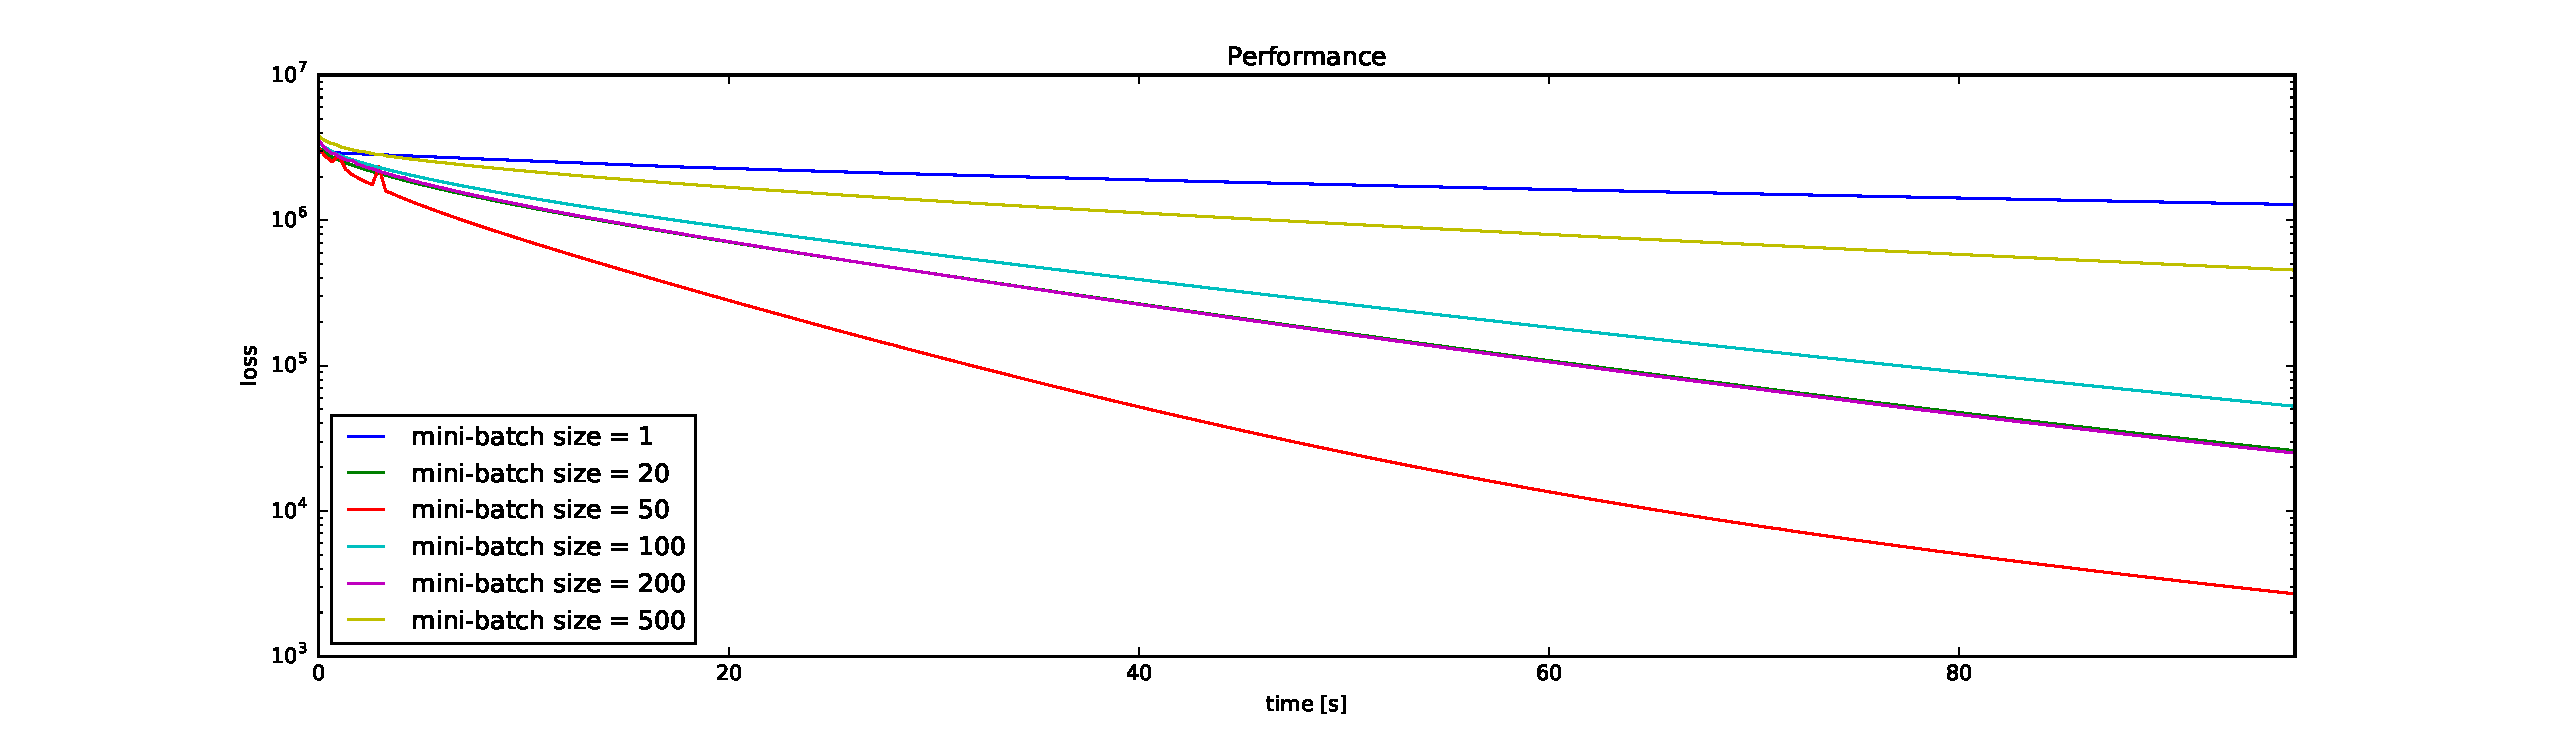
\includegraphics[height=4cm,width=12cm]{figs/perf}}
	\caption{Performance evaluations of mini-batch SAGA w.r.t. various
	mini-batch sizes $m$.}
	\label{fig:eval_saga_mb}
\end{figure*}

\section{Distributed SAGA}

\begin{figure*}[ht]
	\centering
	\subfigure[First variant.]{
		\label{fig:architecture_1}
		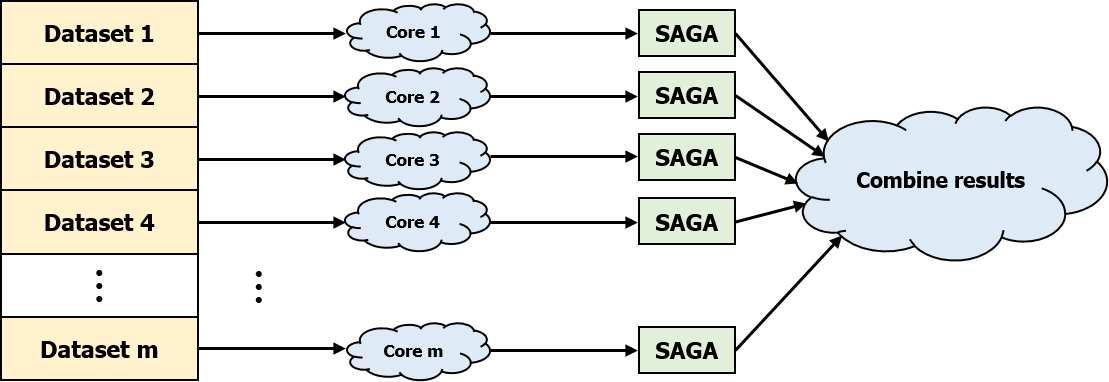
\includegraphics[height=3cm,width=0.48\columnwidth]{figs/architecture_1}}
	\hspace{0pt}
	\subfigure[Second variant.]{
		\label{fig:architecture_2}
		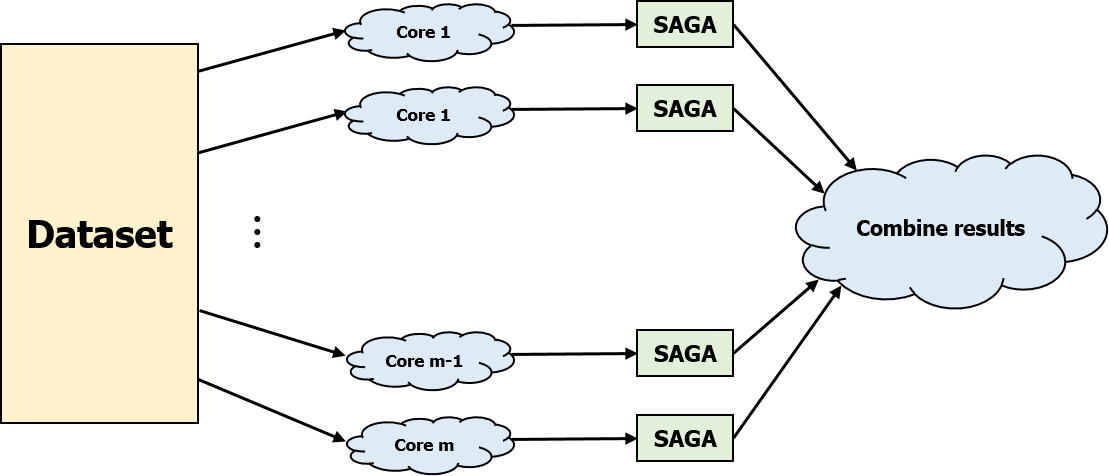
\includegraphics[height=3cm,width=0.48\columnwidth]{figs/architecture_2}}
	\caption{Two variants of distributed SAGA.}
	\label{2figs-show}
\end{figure*}

\paragraph{Variant I.} A first approach, shown in \figref{architecture_1}, is to
randomly partition the $n$ data points onto $m$ machines with $n/m$ local data
points on each to parallelize the computation of \eqnref{saga}. Formally
speaking, at each epoch, we first randomly partition the data into $m$ different
sets. We then apply the SAGA algorithm presented in Section~\ref{sec1} for each
dataset on $m$ different machine. After one pass over each subset, the results
are combined by updating the gradient table and candidate solution. The updates
for epoch $e$ for each $k+1$ then become:
\begin{enumerate}
	\item Randomly partition the dataset into $m$ non-overlapping sets $R_1,
		\cdots, R_m$.
	\item For each machine $s \in \{ 1, \cdots, m \}$, pick a random sample
		$x^k(s)$ from $R_s$.
	\begin{enumerate}
		\item If $ k = 1 $ then $x^k(s) = x(e)$.
		\item Take $\phi_j^{k+1}(s) = x^k(s)$.
		\item Update $x^{k+1}(s) = \prox_\gamma^h \left\{ 
			x^k(s) - \gamma \left[ f_j'(\phi_j^{k+1}(s)) - f_j'(\phi_j^k(s))
			+ \frac1n \sum_{j \in R_i} f_j'(\phi_j^k(s)) \right] \right\}.$
		\item If $ k > n/m$, break.
		\item $k = k+1$.
	\end{enumerate}	
	\item Merge the results with $ x(e+1) = \frac{1}{m} \sum_{s=1}^m x^k(s)$.
\end{enumerate}

\paragraph{Variant II.} A second approach, shown in \figref{architecture_2},
is to randomly pick $m$ data points and send one to each of the $m$ machines.
Each machine then computes \eqnref{saga} in parallel. All results are finally
averaged. The updates for iteration $k+1$ then become:
\begin{enumerate}	
	\item For each machine $s \in \{ 1, \cdots, m \}$
	\begin{enumerate}
		\item Pick a random number $j$ in $[1, n]$.
		\item Take $\phi_j^{k+1}(s) = x^k(s)$, and store $f_j'(\phi_j^{k+1}(s))$
			in the table.
		\item Update $x^{k+1}(s) = \prox_\gamma^h \left\{
			x^k(s) - \gamma \left[ f_j'(\phi_j^{k+1}(s)) - f_j'(\phi_j^k(s))
			+ \frac1n \sum_{i=1}^n f_i'(\phi_i^k(s)) \right] \right\}.$
	\end{enumerate}
	\item Merge the results with $ x^{k+1} = \frac{1}{m} \sum_{s=1}^m
		x^{k+1}(s)$.
\end{enumerate}

\subsection{Experiments}

In this experiment, we set the $\ell_2$ regularization factor to $5\times
10^{-4}$ while we use $n=10^4$ training samples and $m=8$ different machines (or
CPU cores). \figref{distributed_perf} shows the performance of our distributed
methods. A good choice of learning rate, as for all gradient methods, is crucial
as shown in \figref{arch1_lr} and \figref{arch2_lr}. Moreover,
\figref{arch2_par} presents the required time for 1000 iterations using
different models, namely using parfor loop which is the pure distributed
implementation, for loop which is a serial implementation, and vectorized
implementation which relies on parallel implementation of linear algebra
libraries in MATLAB. The results show an heavy communication overhead for
parfor.

\begin{figure*}[ht]
	\centering
	\subfigure[Variant I: learning rate.]{
		\label{fig:arch1_lr}
		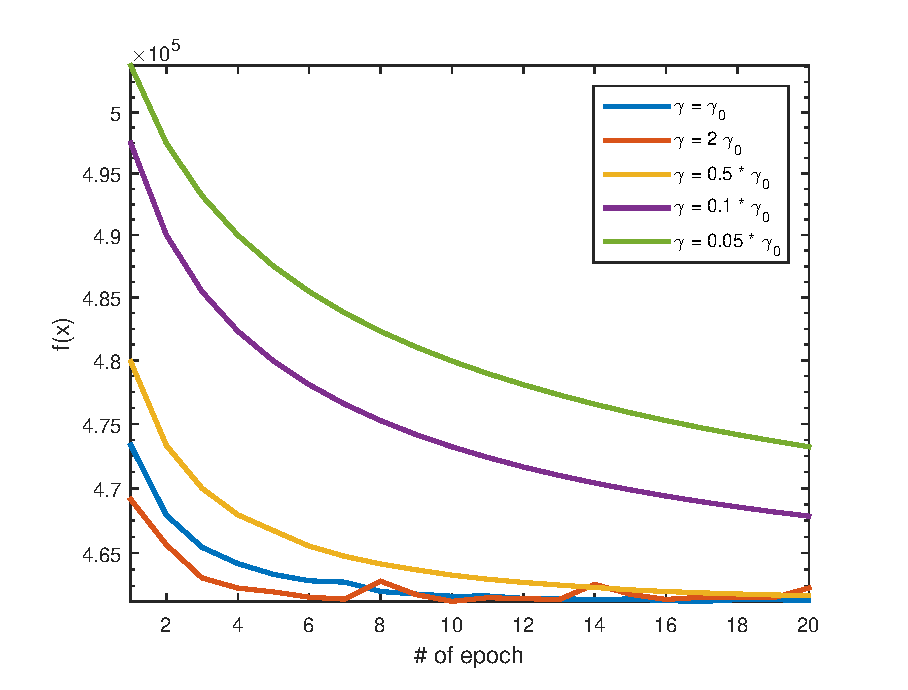
\includegraphics[width=0.31\columnwidth]{figs/arch1_lr.eps}}
	\hspace{0pt}
	\subfigure[Variant II: different parallelizations.]{
		\label{fig:arch2_par}
		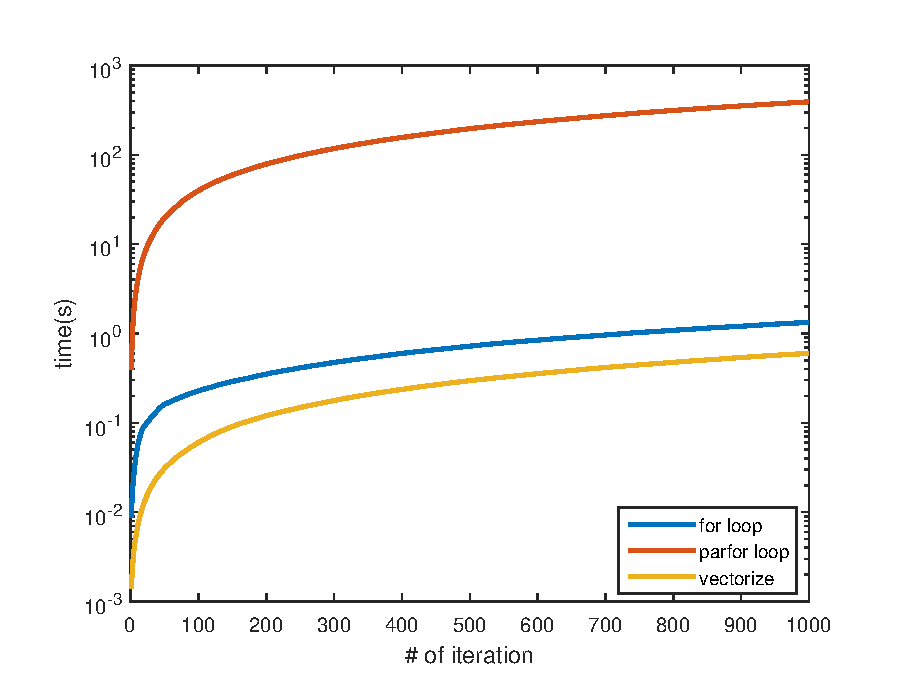
\includegraphics[width=0.31\columnwidth]{figs/arch2_par.eps}}
	\hspace{0pt}
	\subfigure[Variant II: learning rate.]{
		\label{fig:arch2_lr}
		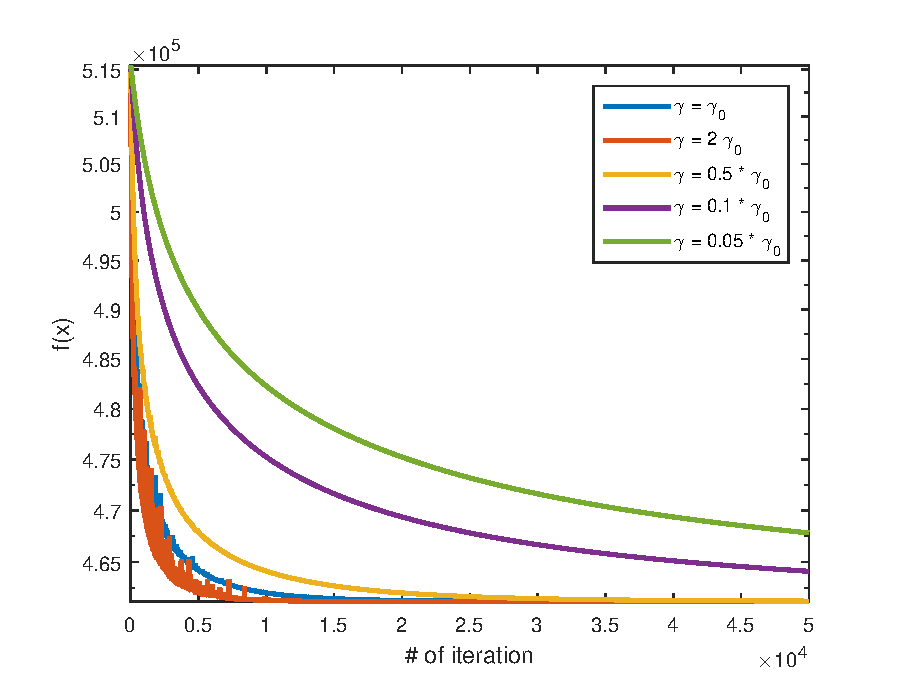
\includegraphics[width=0.31\columnwidth]{figs/arch2_lr.eps}}
	\caption{Performance measures of distributed SAGA.}
	\label{fig:distributed_perf}
\end{figure*}

\figref{conv} compares the two proposed approaches in term of convergence
rate. Variant I converges faster in running time while variant II converges
faster in the number of iterations.

\begin{figure*}[ht]
	\centering
	\subfigure[Convergence w.r.t. the number of iterations.]{
		\label{fig:conv_iterations}
		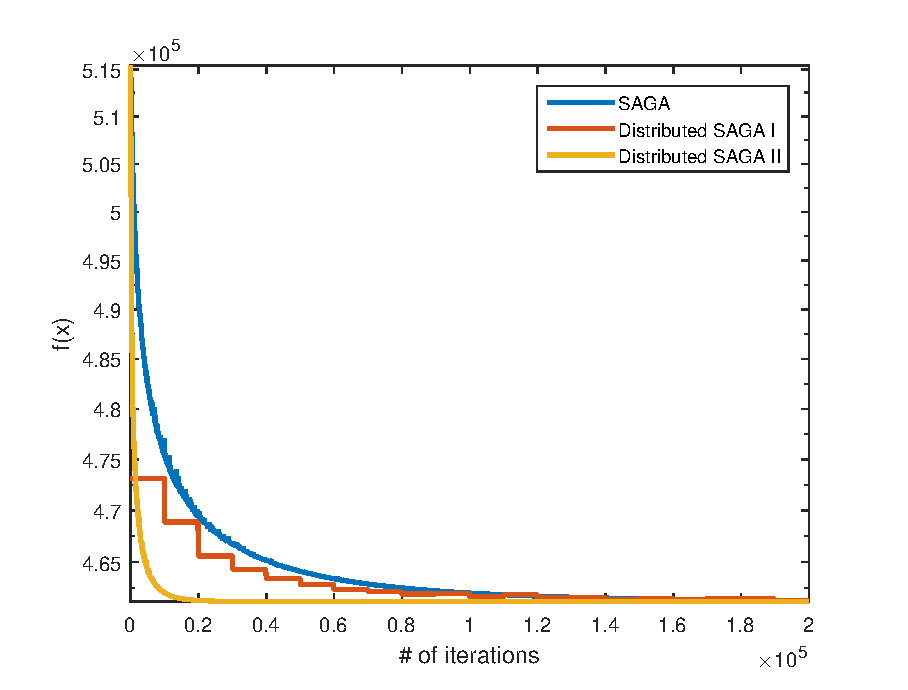
\includegraphics[width=0.31\columnwidth]{figs/conv_iterations.eps}}
	\hspace{0pt}
	\subfigure[Convergence w.r.t. running time.]{
		\label{fig:conv_time}
		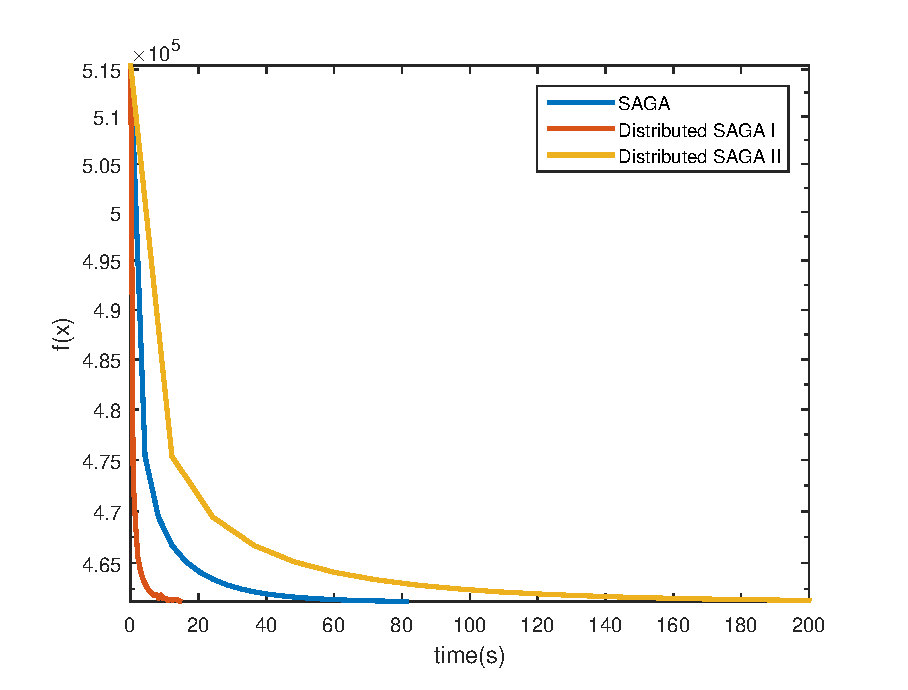
\includegraphics[width=0.31\columnwidth]{figs/conv_time.eps}}
	\caption{Comparison between two distributed SAGA algorithms and regular SAGA.}
	\label{fig:conv}
\end{figure*}

\bibliography{refs}
\bibliographystyle{abbrv}

\end{document}
